% file: 3-2-amortized-analysis/splay-tree-case-I.tex

\documentclass[tikz]{standalone}

\usepackage{tikz-qtree}
\usetikzlibrary{positioning, shapes.geometric}

\begin{document}
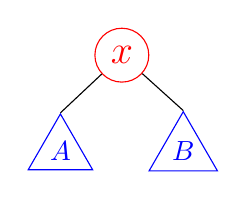
\begin{tikzpicture}[level distance = 35pt, sibling distance = 20pt,
  edge from parent/.style = {
  	draw, edge from parent path = {(\tikzparentnode) -- (\tikzchildnode.north)}}]
  \tikzset{every internal node/.style = {draw, circle, red, font = \Large}}
  \tikzset{every leaf node/.style = {draw, blue, regular polygon, regular polygon sides = 3, inner sep = 1pt}}

  \Tree [.$x$ 
	  $A$
	  $B$
	]
\end{tikzpicture}
\end{document}
